%!TEX root = ./workbook-2014.tex

\section{Writing Functions in Python}

So far we've been mostly using Python's built in functions. However the power of a
true programming language is the ability to write your own functions.

The general form of an Python function is as follows:

\begin{python}
def funcname(arg1, arg2):
    # body of function
    return result
}
\end{python}
%
To make this concrete, here's an example where we define a function in
the interpreter and then put it to use:
%
\begin{python}
>>> def veclength(x):
...     return np.sqrt(np.dot(x,x))
...
>>> x
array([1, 2, 3, 4, 5])
>>> veclength(x)
7.416198487095663
>>> y
array([ 6,  7,  8,  9, 10])
>>> veclength(y)
18.165902124584949
\end{python}

\subsection{Putting Python functions in module}

When you define a function at the interactive prompt and then close the
interpreter your function definition will be lost. The simple way around
this is to define your Python functions in a module that you can than access
at any time.

In your programmer's editor of choice, create a new blank document. Enter your function into the editor
and upload the source file to your virtual machine with a name like
\lstinline!vecgeom.py!.

\begin{python}
# functions defined in vecgeom.py

# this import statement is necessary for the module to use
# functions defined in numpy

import numpy as np

def veclength(x):
    """ Given a numeric vector, returns length of that vector. """
    return np.sqrt(np.dot(x,x))


def unitvector(x):
    """ Return a unit vector in the same direction as x. """
    return x/veclength(x)


\end{python}
There are two functions defined above, one of which calls the other. Both take single vector arguments. These functions have no error checking to insure that the arguments passed to the functions are reasonable but Python's built in error handling will do just fine for most cases.

Once your functions are in a script file you can make them accesible by
using the \lstinline!import()! function:
%
\begin{python}
>>> import vecgeom
>>> x = np.array((1, 0.4))
>>> vecgeom.veclength(x)
1.077032961426901
>>> ux = vecgeom.unitvector(x)
>>> ux
array([ 0.92847669,  0.37139068])
>>> a = np.array([1,2,3,4])
>>> from vecgeom import veclength, unitvector
>>> ua = unitvector(a)
>>> ua
array([ 0.18257419,  0.36514837,  0.54772256,  0.73029674])
>>> veclength(ua)  # how come this value isn't exactly 1.0 as expected?
0.99999999999999989
\end{python}
Note that our functions work with vectors of arbitrary dimension.


\begin{assignment}
Write a function that uses the dot product and the \lstinline!acos()! function to calculate the angle (in radians) between two vectors of arbitrary dimension.  By default, your function should return the angle in radians. Also include a logical (Boolean) argument that will return the answer in degrees.  Test your function with the following two vectors: \lstinline!x = [-3, -3, -1, -1, 0, 0, 1, 2, 2, 3]! and
\lstinline!y = [-8, -5, -3, 0, -1, 0, 5, 1, 6, 5]!.  The expected angle for these test vectors is 0.441 radians (25.3 degrees).
\end{assignment}


Let's also add the following function to |vecgeom.py| to aid in visualizaing 2D vectors:
%
\begin{python}

from matplotlib import pyplot as plt

def draw_vectors(a, b, colors=('red', 'blue'), clear = True):
    """ Given vectors a and b, draw their geometric representation. """"
    # figure out the limits such that the origin and the vector
    # end points are all included in the plot
    xhi = max(0, a[0], b[0])
    xlo = min(0, a[0], b[0])
    yhi = max(0, a[1], b[1])
    ylo = min(0, a[1], b[1])

    xlims = np.array((xlo, xhi))*1.10 # give a little breathing space around vectors
    ylims = np.array((ylo, yhi))*1.10

    if clear:
        ax = plt.axes()
        plt.xlim(*xlims)
        plt.ylim(*ylims)
        plt.xlabel("x-coord")
        plt.ylabel("y-coord")

    plt.arrow(0, 0, a[0], a[1], color=colors[0])
    plt.arrow(0, 0, b[0], b[1], color=colors[1])

\end{python}
%
You can use this new function as follows:
\begin{python}
# if a module has been loaded once, and then you change it
# you must reload the module for the changes to take effect
>>> reload(vecgeom)  
<module 'vecgeom' from 'vecgeom.pyc'>
>>> x = np.array((1, 0.4))
>>> y = np.array((0.2,0.8))
>>> vecgeom.draw_vectors(x,y)
\end{python}
%
The resulting figure should resemble the one below.
%
\begin{figure}[htbp]
\centering
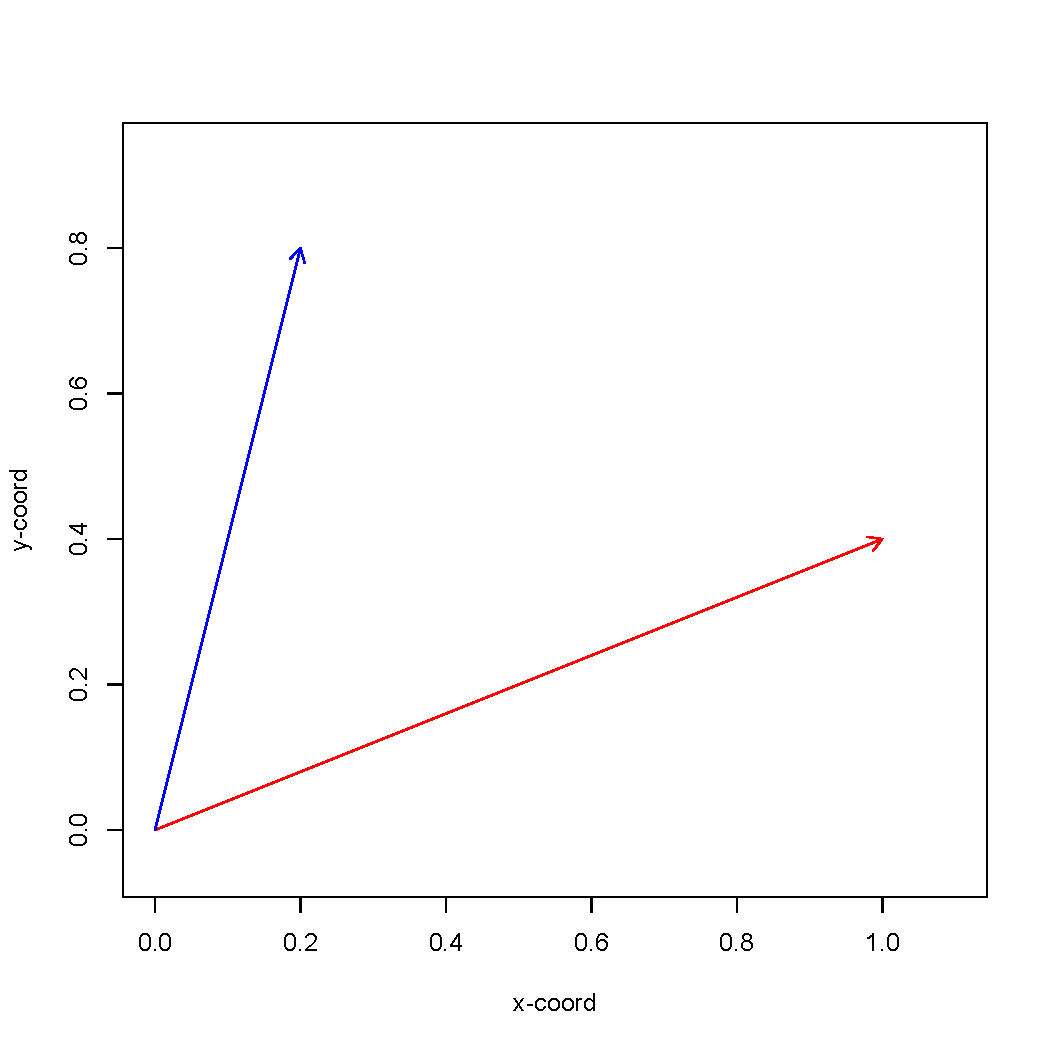
\includegraphics[width=0.33\columnwidth]{./figures/hands-on2/vecfig2.pdf}
\caption{Another vector figure.}
\end{figure}

Notice that we included a |clear| argument in our |draw_vectors| function. I included this so we could add additional vectors to our plot, without overwriting the old vectors, as demonstrated below:
\begin{python}
>>> ux = vecgeom.unitvector(x)
>>> uy = vecgeom.unitvector(y)
>>> vecgeom.draw_vectors(ux, ux, colors=['black','green'], clear=False)
>>> ## you might have to change xlim and ylim
\end{python}
%
Unlike the other functions we wrote, |draw_vectors| only works properly with 2D vectors. Since any pair of vectors defines a plane, it is possible to generalize this function to work with arbitrary pairs of vectors.


\begin{assignment}
Write a function, |vproj()|, that takes two vectors, $\vec{x}$ and $\vec{y}$, and returns a list containing the projection of $\vec{y}$ on $\vec{x}$ and the component of $\vec{y}$ in $\vec{x}$:

\lstDeleteShortInline|

\[P_{\vec{x}}(\vec{y}) = \left(\frac{\vec{x} \cdot \vec{y}}{|\vec{x}|}\right) \frac{\vec{x}}{|\vec{x}|}\]
and
\[C_{\vec{x}}(\vec{y}) = \frac{\vec{x} \cdot \vec{y}}{|\vec{x}|}\]

\lstMakeShortInline|
Use the test vectors from Assignment 2.1 to test your function.  The list returned by your function for these test vectors should resemble that shown below:
%
\begin{python}
>>>> vproj(x, y)
[array([-6, -6, -2, -2, 0, 0, 2, 4, 4, 6]), 12.32883] 
\end{python}
\end{assignment}

